\documentclass{book}

\usepackage[letterpaper]{geometry}
\usepackage{tgpagella}
\usepackage{amsmath}
\usepackage{amssymb}
\usepackage{amsthm}
\usepackage{tikz}
\usepackage{minted}
\usepackage{physics}
\usepackage{siunitx}

\sisetup{detect-all}
\newtheorem{plm}{Problem}

\title{Algebra in Action}
\author{Duncan Wilkie}
\date{21 November 2023}

\begin{document}

\maketitle

\chapter{Preface}

\textit{If you don't know algebra yet, skip to the roadmap; prefaces are directed at people assigning books.}
\vspace{20pt}

This book stems from a divine revelation I had while studying the frightening connections
between modules over field-valued polynomial rings and linear algebra in the wee hours of a morning my senior year of undergrad.
A Discord math friend had demonstrated the clear inadequacy of the geometric intuition for the determinant of a linear transformation,
and posed the question of an algebraic motivation for it.
Toiling over Dummit and Foote's approach to the structure theory of modules at the time, I quickly found the answer:
the product of the roots of the largest invariant factor of the underlying vector space, represented as a module over the polynomial ring
with coefficients in the underlying field where the transformation is replaced by an indeterminate.

This, alongside the spookily elementary proofs of the Jordan and rational canonical form theorems,
threatened my foundational understanding of linear algebra, begotten of Axler's text \textit{par excellence}.
Surely, despite immediate motivation for the most fundamental concepts emerging from deepest depths, there's something more to linear algebra?
Could it really be, fundamentally, the study of structures over polynomial rings?

Thinking over how one might deface Axler in this light brought a new perspective on the whole of algebra.
You're given a vector space $V$ over a field $F$, and a linear operator on it, $T$.
What can you do, without giving $V$ the standard agonizing vivisection?
Well, you can add any operator expression to any other, via pointwise addition in the vector space,
and you can borrow $V$'s scalar multiplication similarly.
You can also compose $T$ with itself, forming ``powers'' of $T$.
To the initiated, it's clear this is all just a consequence of viewing the endomorphism ring of $V$ as a module.
But, that's not so obvious a perspective \textit{ab initio}.
Pondering how to justify considering composition of $T$ as ``multiplication,'' it dawned on me that
\textit{every other multiplication is actually composition of endomorphisms}.

The attendant emotional consequences are witnessed in the figure.

\begin{center}
  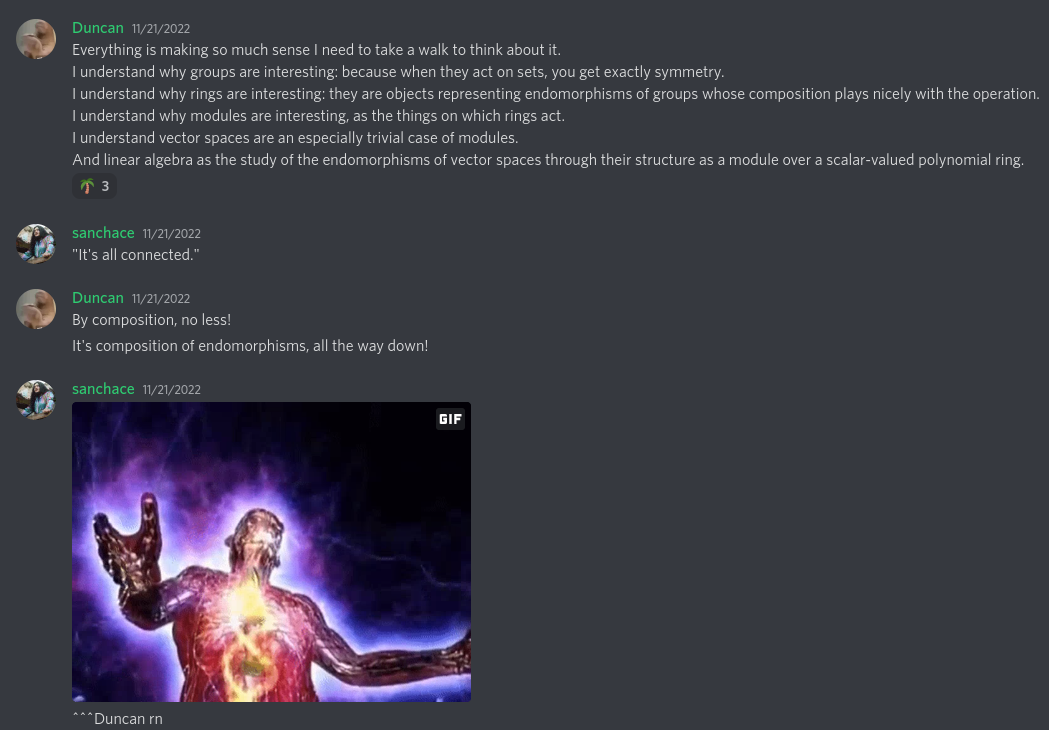
\includegraphics[scale=0.3]{galaxy_brain.png}
\end{center}

This provided an intuitive justification for all my hard-won opinions on proper conventions (e.g. rings not rngs, 0 is a natural number),
explained definitions that seemed to fall from the sky (associativity, distributivity, rings are Abelian groups),
and provides a more palatable hint towards category theory than ``it's what we need to describe functors which are what we need to describe
natural transformations.''

Practically, this text seeks to be a first course in modern (abstract) algebra from a categorical perspective,
correcting the gaps in motivation left by the laudable recent treatments with the same goal. % TODO: Cite Aluffi and D\&F
The only prerequisite is an introduction to proofs class covering basic set theory, such as \textit{Book of Proof} or the first chapter of Munkres.
The results used are summarized in an appendix.

I produce also machine-verified proofs of each result, as an aid in my writing clear and concise arguments
and a recourse for the logically-minded reader peeved by my omission of trivial results, or suspicious of my wording.
They are in Lean 4, and are in print separately, in addition to freely distributed online.
I have made painstaking attempts to establish everything constructively, and any thus-intractable proof is distinguished by (a symbol) % TOOD: pick
and the nonconstructive step is identified in the text.

\chapter{Roadmap}
The text is organized into two parts: theory and application.
The first is entirely self-contained, containing pure algebra.
% TODO: list of chapters
\begin{enumerate}
\item Todo
\end{enumerate}
The second draws on the theory through established applications elsewhere, in a linear fashion
(within chapters, section numbers $\propto$ theory chapter numbers).
% TODO: list of chapters
\begin{enumerate}
\item Todo
\end{enumerate}
You can pick one you like, for examples of how these concepts are absolutely critical for the ``real world'' as you define it.

Here's a section-level dependency graph of the theorems save basic set theory and logic:

For mathematicians: a reasonable path for an undergraduate first course in algebra is the group chapters alone.
For a two-semester sequence, the standard groups-rings-fields approach is tried and true.
For more advanced students that have had a year or so of proof-heavy classes, one can supplement the above with the first chapter on categories.
For a graduate-level course, the whole theory part can be done until you run out of time.
Groups $\to$ rings $\to$ modules $\to$ fields is tried-and-true.

For professors of $X$ teaching applied algebra in the $X$ department: pick your favorite algebraic structure, do only it and the basic category theory chapter, and proceed to your corresponding applications chapter.

\tableofcontents



\end{document}
